\documentclass[border=2mm]{standalone}
\usepackage{tikz}
\usetikzlibrary{positioning}
\usepackage{array}

\definecolor{darkred}{rgb}{0.5, 0.0, 0.0}
\definecolor{darkgreen}{rgb}{0.0, 0.5, 0.0}
\definecolor{darkblue}{rgb}{0.0, 0.0, 0.5}

\begin{document}

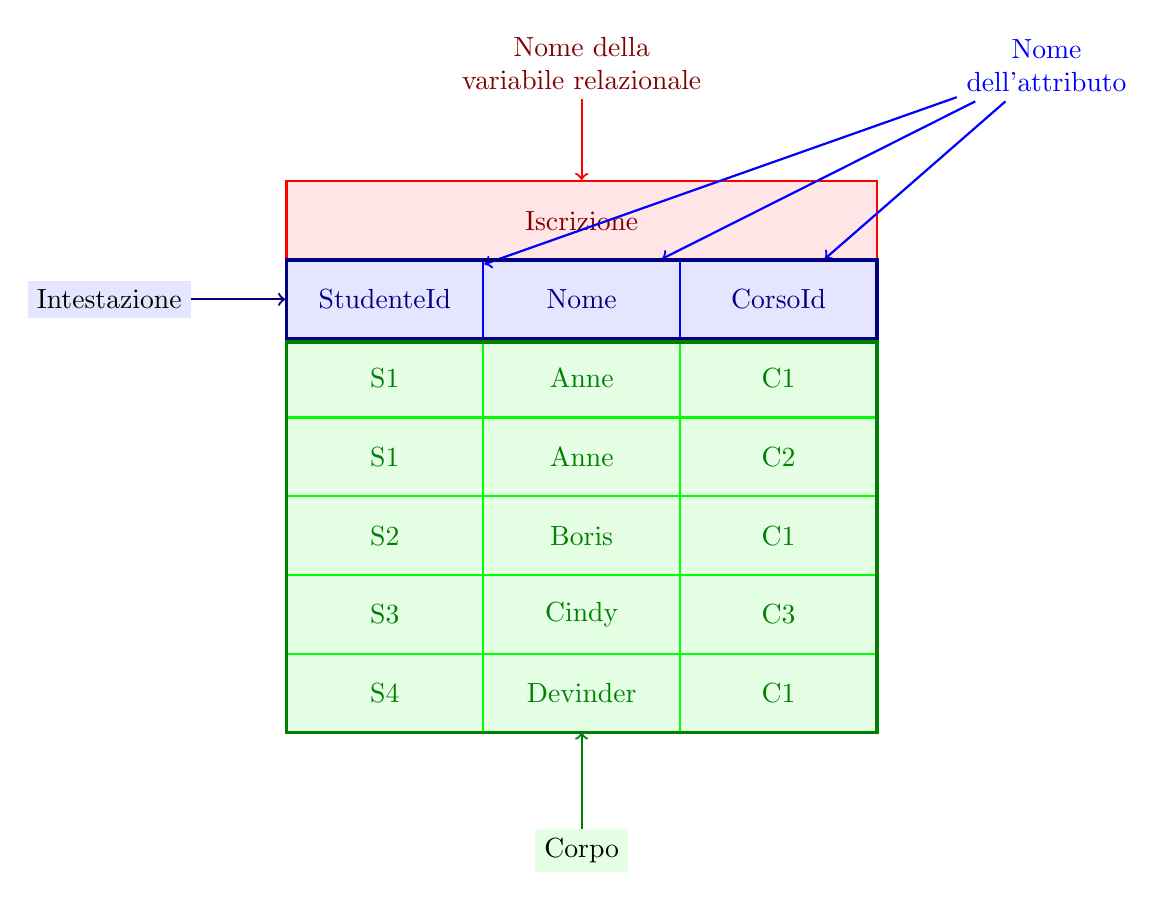
\begin{tikzpicture}
    % Stile per le celle della tabella
    \tikzset{
        table_cell/.style={
            draw=green, % Bordo visibile
            text=darkgreen,
            fill=green!10, % Sfondo
            thick,
            minimum width=2.5cm, % Larghezza minima della cella
            minimum height=1cm, % Altezza minima della cella
            align=center, % Allineamento centrale del testo
            font=\normalsize, % Dimensione del font
            outer sep=0pt, % Rimuove spazio extra intorno al nodo
            inner sep=0.2em % Piccolo spazio interno per il testo
        },
        table_header/.style={
            draw=blue, % Bordo visibile
            text=darkblue,
            fill=blue!10, % Sfondo
            thick,
            minimum width=2.5cm, % Larghezza minima della cella
            minimum height=1cm, % Altezza minima della cella
            align=center, % Allineamento centrale del testo
            font=\normalsize % Dimensione del font
        },
        table_name/.style={
            draw=red, % Bordo visibile
            fill=red!10,
            text=darkred,
            thick,
            minimum width=7.5cm, % Larghezza minima della cella
            minimum height=1cm, % Altezza minima della cella
            align=center, % Allineamento centrale del testo
            font=\normalsize % Dimensione del font
        }
    }

    % Riga del nome della tabella
    \node[table_name] (table_name) at (0,0) {Iscrizione};

    % Intestazioni
    
    \node[table_header] (header1) at (-2.5,-1) {StudenteId};
    \node[table_header] (header2) at (0,-1) {Nome};
    \node[table_header] (header3) at (2.5,-1) {CorsoId};

    
    % Valori
    \node[table_cell] (row1_col1) at (-2.5,-2) {S1};
    \node[table_cell] (row1_col2) at (0,-2) {Anne};
    \node[table_cell] (row1_col3) at (2.5,-2) {C1};

    \node[table_cell] (row2_col1) at (-2.5,-3) {S1};
    \node[table_cell] (row2_col2) at (0,-3) {Anne};
    \node[table_cell] (row2_col3) at (2.5,-3) {C2};

    \node[table_cell] (row3_col1) at (-2.5,-4) {S2};
    \node[table_cell] (row3_col2) at (0,-4) {Boris};
    \node[table_cell] (row3_col3) at (2.5,-4) {C1};

    \node[table_cell] (row4_col1) at (-2.5,-5) {S3};
    \node[table_cell] (row4_col2) at (0,-5) {Cindy};
    \node[table_cell] (row4_col3) at (2.5,-5) {C3};

    \node[table_cell] (row5_col1) at (-2.5,-6) {S4};
    \node[table_cell] (row5_col2) at (0,-6) {Devinder};
    \node[table_cell] (row5_col3) at (2.5,-6) {C1};

    % Annotazioni
    \node[above of=table_name, node distance=2cm,text=darkred,align=center] (note1) {Nome della\\variabile relazionale};
    \draw[->, color=red,thick] (note1) -- (table_name);

    % Per le intestazioni (raggruppamento)
    \node[left of=header1, node distance=3.5cm,fill=blue!10] (note2) {Intestazione};
    \draw[->, color=darkblue,thick] (note2) -- (header1.west); % Freccia generica verso le intestazioni

    % Per i singoli nomi degli attributi (richiede più frecce)
    \node[above right = of table_name,text=blue,align=center] (note3) {Nome\\ dell'attributo};
    \draw[->,thick, color=blue] (note3) -- (header1);
    \draw[->,thick, color=blue] (note3) -- (header2);
    \draw[->,thick, color=blue] (note3) -- (header3);

    % Per il corpo della tabella
    \node[below of=row5_col2, node distance=2cm,fill=green!10] (note4) {Corpo};
    \draw[->,color=darkgreen,thick] (note4) -- (row5_col2.south); % Freccia verso il centro del corpo

    % Bordo intestazione
    \draw[color=darkblue, very thick] (-3.75,-1.5) rectangle (3.75,-0.5);
    % Bordo corpo
    \draw[color=darkgreen, very thick] (-3.75,-6.5) rectangle (3.75,-1.54);

\end{tikzpicture}
\end{document}
